\documentclass[tikz, border = 2pt]{standalone}

%---------------------------------------------------------------------------%
% PACKAGES                                                                  %
%---------------------------------------------------------------------------%

%----- MATH
%---------------------------------------------------------------------------%
\usepackage{amsmath, amssymb}

%----- FIGURES
%---------------------------------------------------------------------------%
\usepackage{pgfplots}
\pgfplotsset{compat=1.13}

\begin{document}

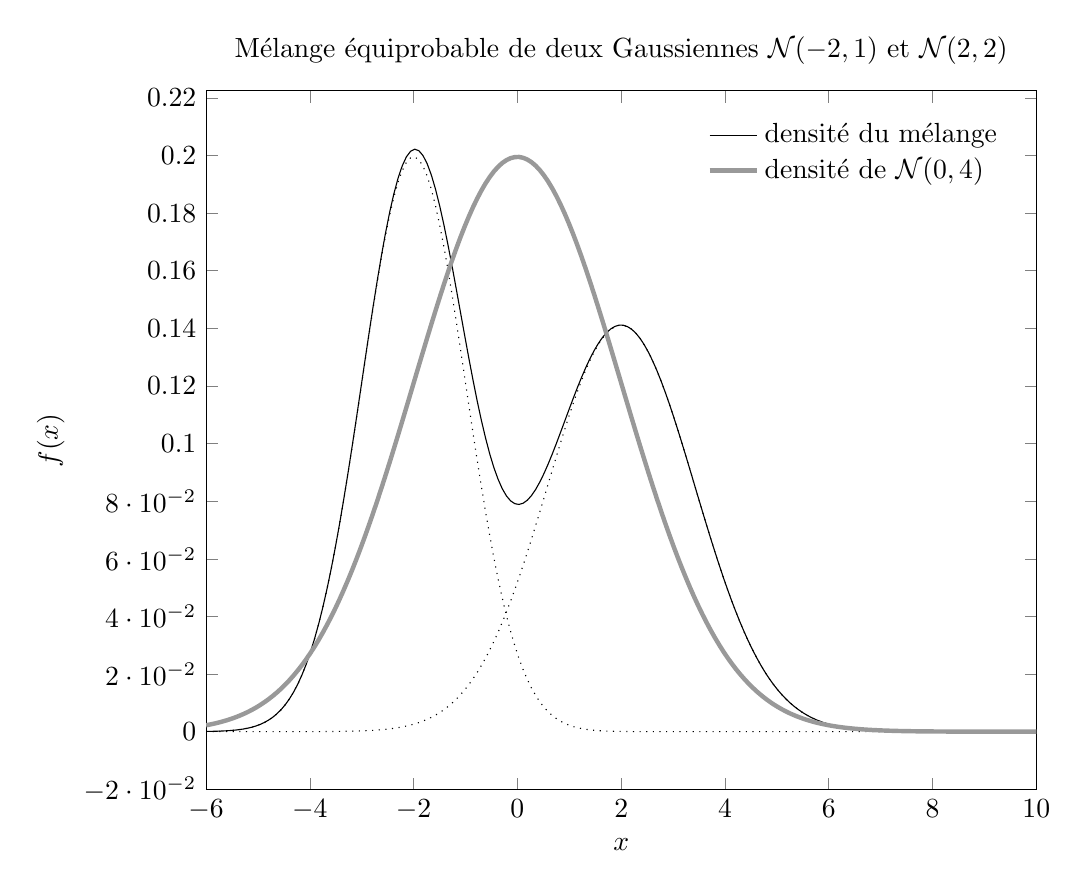
\begin{tikzpicture}
\begin{axis}[width = \textwidth,
title style = {align = center},
title={M\'elange \'equiprobable de deux Gaussiennes $\mathcal{N}(-2,1)$ et $\mathcal{N}(2,2)$},
xlabel={$x$},
ylabel={$f(x)$},
legend pos = north east,
legend style = {draw=none},
legend cell align = left,
xmin = -6,
xmax = 10,
ylabel near ticks,
domain = -6:10
]
\addplot[black, dotted, samples = 200, forget plot] {0.5*(1/sqrt(2*pi))*exp(-(x+2)^2/2)};
%
\addplot[black, dotted, samples = 200, forget plot] {0.5*(1/sqrt(4*pi))*exp(-(x-2)^2/4)};
%
\addplot[black, samples = 200] {0.5*(1/sqrt(2*pi))*exp(-(x+2)^2/2) + 0.5*(1/sqrt(4*pi))*exp(-(x-2)^2/4)};
%
\addplot[black!40, ultra thick, samples = 200] {(1/sqrt(8*pi))*exp(-(x)^2/8)};
%
\legend{{densit\'e du m\'elange}, {densit\'e de $\mathcal{N}(0,4)$}}
\end{axis}
\end{tikzpicture}

\end{document}